% EclipseFP-JE.tex
\begin{hcarentry}{EclipseFP}
\report{JP Moresmau}%11/11
\status{stable, maintained}
\participants{B.\ Scott Michel, Alejandro Serrano, building on code from Thiago Arrais, Leif Frenzel, Thomas ten Cate, and others}
\makeheader

EclipseFP is a set of Eclipse plugins to allow working on Haskell code projects.
It features Cabal integration (.cabal file editor, uses Cabal settings for compilation), and GHC integration. Compilation is done via the GHC API, syntax coloring uses the GHC Lexer. Other standard Eclipse features like code outline, folding, and quick fixes for common errors are also provided. EclipseFP also allows launching GHCi sessions on any module including extensive debugging facilities. It uses Scion to bridge between the Java code for Eclipse and the Haskell APIs.
The source code is fully open source (Eclipse License) and anyone can contribute. Current version is 2.1.0, released in September 2011 and supporting GHC 6.12 and 7.0, and more versions with additional features are planned. Feedback on what is needed is welcome! The website has information on downloading binary releases and getting a copy of the source code. Support and bug tracking is handled through Sourceforge forums.

%**<img width=500 src="./eclipsefp-screenshot1.jpg">
%*ignore
\begin{center}
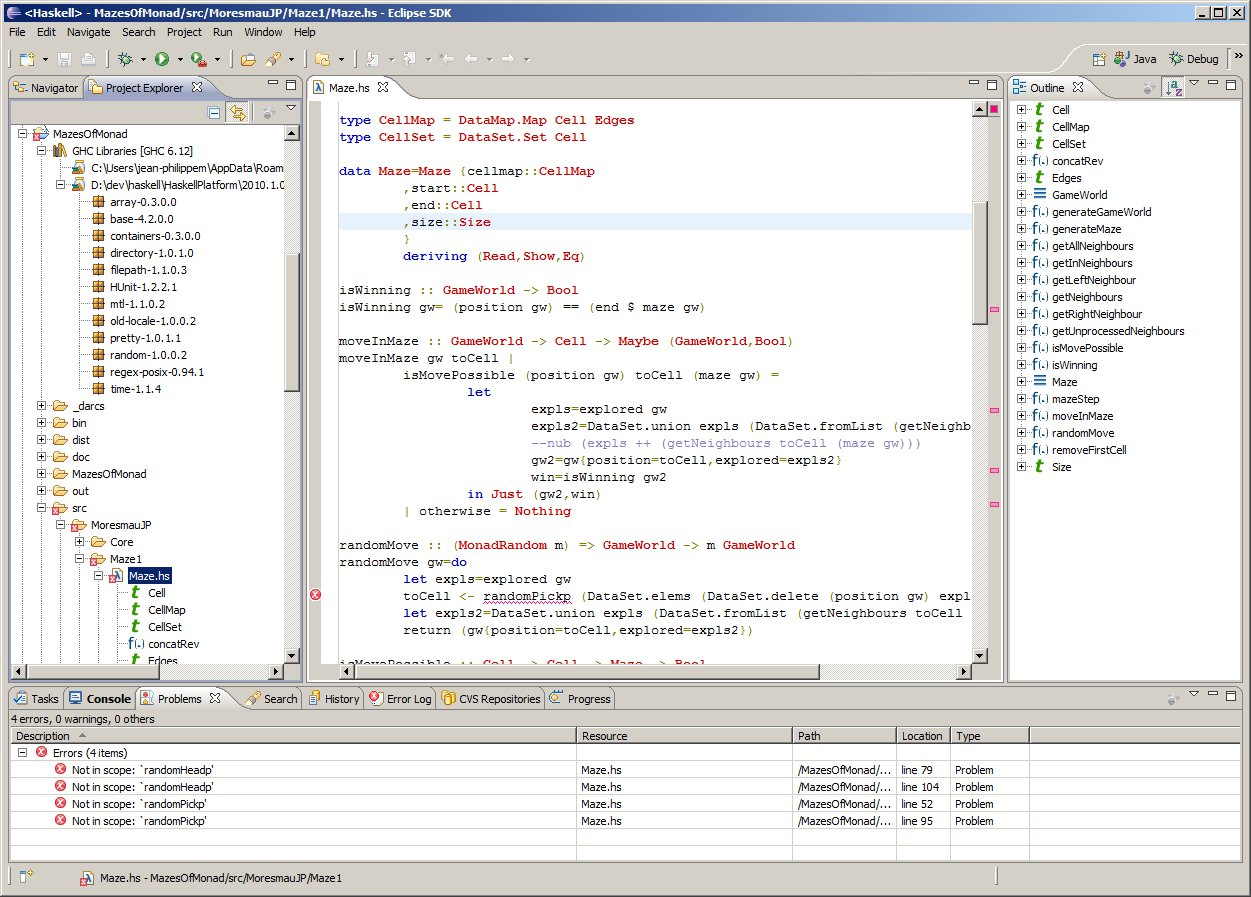
\includegraphics[width=0.47\textwidth]{html/eclipsefp-screenshot1.jpg}
\end{center}
%*endignore

\FurtherReading 
\url{http://eclipsefp.sourceforge.net/}
\end{hcarentry}
